\section{Statistical Models for heterogeneous age groups}
With a full development of statistical rate models for a single age
group behind us, this section turns to a peculiar feature of
population rate meta-analysis: the wide variety of age groups reported
in the literature.

\subsection{Introduction}
A typical example of the heterogeneity in age groups is shown in
Figure~\ref{theory-age_group_model-af_age_groups}.  The middle of the
age group is scattered against the width of the age group.  Simply
put, there is no standard set of age groups for epilepsy research, and
different studies use report results with different age groups.
Unfortunately, this phenomenon is far from unique to epilepsy.

\begin{figure}[h]
\begin{center}
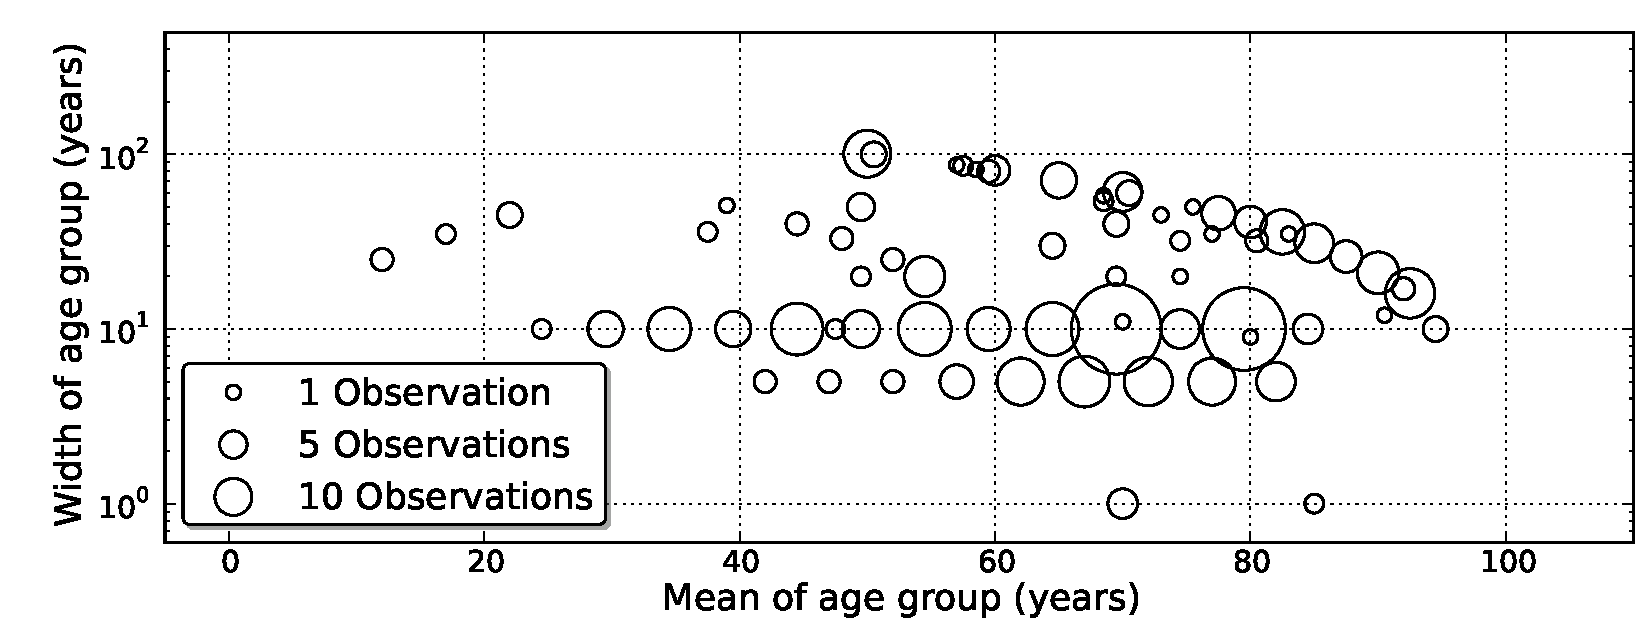
\includegraphics[width=\textwidth]{af_age_groups_scatter.png}
\end{center}
\caption{Mean and spread of age groups in the prevalence data collected
  from a systematic review of epilepsy (jittered to show density).
  There were $<<len(d['af_age_groups.json']['data'])>>$ rows of prevalence
  data extracted, but the most common age
  group accounted for only $<<d['af_age_groups.json']['most_freq_cnt']>>$ rows.}
\label{theory-age_group_model-af_age_groups}
\end{figure}

TK figure showing the heavy-tailed distribution of data count by age group.

This variation in reporting would be no problem if I had access to the
microdata gathered in the course these studies.  From microdata, for
example from a national health information system or from a
demographic household survey, I could simply tally the prevalence
rates by single year age groups.  Although each individual row of data
gathered in this way would have high variability, the rate model from
the last section combined with the age pattern model would do their
work to come up with a combined estimate that is as uncertain as it
should be.

Re-analysis from microdata is occassionally a possibility in a GBD
study, and I expect it to be possible more frequently when in national
and subnational settings.  In the common situation
that the rate microdata is not available, then the rates cannot be
re-tallied into homogeneous, appropriately fine age groups, and an
alternative approach is needed.

There are several statistical approaches which can be employed, and
they will be compared and contrasted in this section.  Before getting
into this, however, it is worthwide to example some of the common
types of age grouping that arise in systematic review.

In the design and dissemination of a study which includes descriptive
epidemiological measurements of population health, there are many
factors that influence the decision of what age groups to include in
analysis.  The authors of each study have often given careful
consideration to the timeless question of scientific research: ``who
do you you want to convince of what?''  And the answer often has
bearing on what age groups are appropriate. TK specific examples.
Even with so proximate a goal as to convince an editor at a journal to
accept a manuscript for publication has implications.  Perhaps age
groups were selected before the study was conducted based on a power
calculation, to be wide enough so that the results can claim
statistical significance.  Perhaps there is a scientific hypothesis
about a risk factor or treatment for the condition of interest and the
study was designed to investigate this hypothesis only for an age
group that seemed most likely to shed light on the tangentially
related question of interest.  Even in a study specifically designed
to measure the age pattern of an epidemiological rate, the age groups
may be selected in an ad hoc manner, based on what researchers running
the study think will be most important or communicative.

Regardless of the factors influencing the decision, there is a simple
mathematical model of what is going on.  The study conducts some sort
of measurement on a population of individuals who are all of different
ages, and then the epidemiological rate or rates of interest are
tallied for age groups selected in some context dependent manner. TK
short rant about using half-open intervals to represent age groups
precisely( TK a note on interval notation, and the way this differs
from traditional demography notation, and how my way will be better
once the reader gets used to it.  ). If the study was a prevalence
study using a full census sample, for example, and if I use
$r_{a_0,a_1}$ to denote the rate for age group $[a_0, a_1)$ and
  $p_{a_0,a_1}$ to denote the subpopulatoin size of age group $[a_0,
    a_1)$, then the identity
\[
p_{a_0, a_2} = p_{a_0,a_1} + p_{a_1,a_2}
\]
says nothing more complicated than that the size of the subpopulation
of age at least $a_0$ and less than $a_2$ is the sum of the size of
the subpopulation between age $a_0$ and $a_1$ and the size of the subpopulation between age $a_1$ and $a_2$.  Applying the same observation to the part of these subpopulations who have the condition of interest yields the following identity
\[
r_{a_0,a_2} = r_{a_0,a_1}p_{a_0,a_1}/p_{a_0,a_2} + r_{a_1,a_2}p_{a_1,a_2}/p_{a_0,a_2}.
\]
In a limiting case of an very large population with very fine age intervals, this becomes
\[
r_{a_0,a_2} = \int_{=a_0}^{a_2} r_{a,a+da}p_{a,a+da}/p_{a_0,a_2}
\]
Undoubtedly all real studies are more complicated than this full
census of prevalence, but this is a starting point for conceptualizing
where age-grouped rates come from.  Roughly, they are integrals over
instantanious rates for infinitesimal age groups.

\subsection{Overlapping age group data}
This section explores several examples of overlapping age group data
collected in systematic reviews, through graphical statistics.  The
primary way I like to display overlapping age-group data is shown in
Figure~\ref{theory-age_group_model-dismod_data_plot}, as horizontal
lines on a plot of age versus rate value.  The level of the bars shows
the rate value, while the width of the bars shows the range of ages
included in the age group. It is possible to augment these lines with
error bars, showing the uncertainty reported for each rate value, but
for this section I have left out the representation of uncertainty, to
keep the plots as simple as possible.

\begin{figure}[ht]
\caption{TK slow description of the dismod data plot,
showing large age group data and small age group data.}
\label{theory-age_group_model-dismod_data_plot}.
\end{figure}

TK Some additional examples of dismod data plots from real data for
certain countries, regions, etc. Hep C from North America High
Income. Anxiety from Subsaharan Africa East.  Cannabis Use, etc.

With a firm understanding of the sort of overlapping age group data
that arises in systematic review, I now turn to developing and
analysing a series of models for the meta-analysis of the data.

\subsection{Midpoint model}
The simplest approach to modeling data with heterogeneous age
intervals, which is often used in practice [refs TK], is to apply each
rate measurement to the midpoint of the age group it measured.  This
is trivial operationally, but it is also theoretically justified
through a ``trapazoidal rule'' integration which will be developed
below in concert with a more elaborate approach.

In practice, this approach works quite accurately for modeling a
disease rate which changes slowly as a function of age.  However, it
becomes quite inaccurate when modeling rates which change more
rapidly.  The typical setting in applications in Chapters TK
will include a few studies which focus on age patterns and hence have
narrow age groups, together with a lot of other studies which focus on
other aspects of disease epidemiology.  Thus the relevant setting to
consider how these models are inaccurate is where three are a few
small-age-group studies and many large-age-group studies.

TK example of how this works out, using good notation from above to
get a formal statistical model specified, and also using age pattern
prior from to-be-written section which should proceed this one.
\begin{align*}
r_i &\sim \NegativeBinomial(\pi_i, \delta_i)\\
\pi_i &= f(\overline{a_i})\\
\log_{10}(\delta_i - 5) &\sim \Normal(\log\delta, .25^2)\\
\log f &\sim \GP(0, \calC)\\
\calC &= 2 + \Matern(10, 2, \rho)
\end{align*}

TK dismod data plot of simulated data, together with an estimate using
appropriately selected age dummies?  This requires developing prior on
age functions.

Discussion of typical approach, using the midpoint of the age range is
the level:
For example in print: \url{
  http://www.rachel.org/lib/meta_leukemias_near_nukes.070701.pdf }

\subsection{Disaggregation}
An alternative to the midpoint model which seems appealing but has
some downsides is what I call disaggregation.  This approach is an
attempt to simulate the re-analysis which could be done if microdata
was available that I described at the beginning of this section.  If
there is no microdata available, I could still hope to disaggregate
the age groups into a refined grouping that is compatible with all
studies collected during the systematic review (1-year age groups, for
example).  This requires taking into account the increased variation
that would be found if a study of the same size was reported for finer
age groups.  Without any additional information, rate data reporting a
level of $r$ for a population of size $n$ for age group $[a_0,a_1)$,
  i.e.,
\[
X = (r, n, a_0, a_1)
\]
can be disaggregated into $A = a_1-a_0$ rows of data, $X_1, X_2,
\ldots, X_A$, with
\[
X_a = (r, \frac{n}{a_1-a_0}, a, a+1), \text{for } a=1,2,\ldots,A.
\]

Disaggregation can  be interpreted as a data preprocessing step, and
this disaggregated data can be fed to the midpoint model from the
previous section to produce a comprehensive estimate of the rate as a
function of age.

However, this model has some unintended negative features when large
age intervals are disaggregated.  It tends to over-compress age
patterns at young and old ages, as shown in Figure TK.

TK figure showing the effects of fitting a model with this
disaggregation approach to the same simulated data shown in the
midpoint example above.

\subsection{Midpoint model with group width covariate}
An alternative approach, which I consider more ``statistical''
culturally is to add the width of the age group as a covariate into
the midpoint model.  This model takes the form
\begin{align*}
r_i &\sim \NegativeBinomial(\pi_i, \delta_i)\\
\pi_i &= f(\overline{a_i}) + \beta_0 + \beta_1 A_i\\
\delta_i &= \gamma_0 + \gamma_1 A_i
\end{align*}
TK description of the $\beta$ and $\gamma$ terms in this model.

This addresses the shortcomings of the disaggregation approach
\emph{indirectly}, and the indirect nature has positives and
negatives.  This approach does not explicitly connect the large age
interval to the small interval, but instead allows the data to inform
the relationship.  On the other hand, it posits that the data-driven
relationship between the rates for studies with the same midpoint but
different age groups is a linear relationship, while the mathematical
model developed at the beginning of this section for how the rate of
an age group is measured is ``nonlinear'' in a specific and
mechanistically known way.

TK graphic showing the midpoint model at work.

\subsection{Age-integrating models}
An even more complicated approach, both conceptually and
computationally, is to average across the age interval explicitly in
the statistical model.
\begin{align*}
r_i &\sim \NegativeBinomial(\pi_i, \delta_i)\\
\pi_i &= \int_{a=a0_i}^{a1_i} f(a)dw(a),
\end{align*}
where the integration $dw$ is weighted according to population
structure.

This has the theoretical appeal of matching the generative model above
by the drawback of being slower to compute and less stable numerically
(to be investigated in detail in Chapter TK).  It also has a major
piece left unspecified, the selection of the age weights for the
integration.  There are two sensible approaches to this, which I call
the \emph{age-standardizing model}, where a common age pattern is used
for all studies and the \emph{age-averaging model}, where the best
estimate available of the age pattern of the study population is
used.  The age-standardizing model is faster, due to a computational
optimization to be developed in Chapter TK, but the age-averaging
model has a certain theoretical appeal because it uses the best
information available.  However it is not certain that using this
information will make the end results any more accurate, because the
age pattern of the study population is rarely know with much
certainty, and often it is necessary to assume that it matches the
national age pattern for the country-years where the study was
conducted.  In the case of remission and mortality studies it is even
more complicated to estimate the study population age pattern, since
it is \emph{not} the same as the national population age pattern, but
modulated by the age pattern of disease prevalence.

TK comparison of the various approaches on synthetic data.

\section{Model comparison}
An appropriate comparison of these approaches is somewhat difficult to
develop.  One approach is through simulation study, but this risks
inappropriate model selection due to inaccurately choosing the
distribution of the simulated data.  A better approach is
cross-validatoin, TK description of that I mean by that.  Naively
holding out $25\%$ of the data doesn't address the exact topic of
interest, however, since it determines which model predicts rates of
all age groups, and I am really only interested in predicting the age
groups with small widths accurately.  It would be preferable to hold
out only data with small-width age groups from large representative
subpopulations.  Unfortunately three is rarely enough data to do this,
especially in all the settings that come up in disease modelsing.

I have taken a pragmatic approach, evaluating with a variety of
simulations and cross-validatoins, described now:

TK a description of a combination of approaches:

1) Fit real data to get ``truth''

2) Simulate from truth to get sim data, with random age intervals or
with age intervals taken from a real dataset

3) Fit sim data and calculate RMSE and prob cov

Holdout cross-validatoin:  Choose 25\% of data to hold out, uniformly
or only from high quality data.  Fit, compare observation and
prediction.

Summary of results:  many similarities from all models, although it is
clear that the midpoint model is wrong and the disaggregated midpoint
model is even worse.

For future research, I would like to use cross-validation to select
the best age group model on a case-by-case basis.  This could adapt
the ensemble approach used in CoDMod, where an average of results from
all the different models was computed based on using cross-validatoin
to decide how much weight each model should be given.
